\begin{titlepage}
\begin{center}
    \textbf{PROPOSAL MBKM RISET}\\[3\baselineskip]

    %research title
    \textbf{PENGEMBANGAN MODEL DETEKSI DAN KLASIFIKASI OBYEK DENGAN DETECTOR BERBASIS ARSITEKTUR CONVOLUTIONAL NEURAL NETWORK UNTUK MENDUKUNG PARIWISATA HALAL}\\[8\baselineskip]

    %university logo
    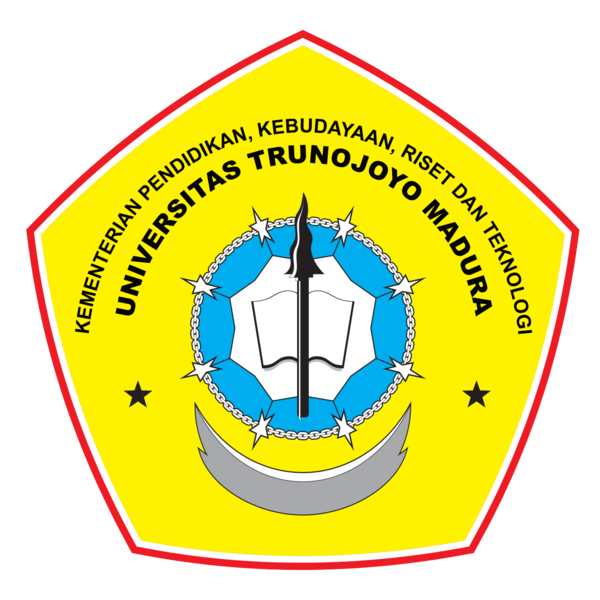
\includegraphics[width=3.5cm, height=3.5cm]{UTM_DIKBUDRISTEK}\\[3\baselineskip]

    %author
    Disusun Oleh:\\
    Robby Alamsyah NIM. 190411100046\\[1\baselineskip]

    %mentor
    Dibimbing Oleh:\\
    Dr. Indah Agustien Siradjuddin, S. Kom, M. Kom. NIDN. 0020087803\\[8\baselineskip]


    \textbf{LEMBAGA PENELITIAN DAN PENGABDIAN KEPADA MASYARAKAT}\\
    \textbf{UNIVERSITAS TRUNOJOYO MADURA}\\
    \textbf{BANGKALAN}\\
    \textbf{SEPTEMBER 2022}
\end{center}
\end{titlepage}